% !TeX program = pdfLaTeX
\documentclass[12pt]{article}
\usepackage{amsmath}
\usepackage{graphicx,psfrag,epsf}
\usepackage{enumerate}
\usepackage{natbib}
\usepackage{textcomp}
\usepackage[hyphens]{url} % not crucial - just used below for the URL
\usepackage{hyperref}
\providecommand{\tightlist}{%
  \setlength{\itemsep}{0pt}\setlength{\parskip}{0pt}}

%\pdfminorversion=4
% NOTE: To produce blinded version, replace "0" with "1" below.
\newcommand{\blind}{0}

% DON'T change margins - should be 1 inch all around.
\addtolength{\oddsidemargin}{-.5in}%
\addtolength{\evensidemargin}{-.5in}%
\addtolength{\textwidth}{1in}%
\addtolength{\textheight}{1.3in}%
\addtolength{\topmargin}{-.8in}%

%% load any required packages here


\usepackage{color}
\usepackage{fancyvrb}
\newcommand{\VerbBar}{|}
\newcommand{\VERB}{\Verb[commandchars=\\\{\}]}
\DefineVerbatimEnvironment{Highlighting}{Verbatim}{commandchars=\\\{\}}
% Add ',fontsize=\small' for more characters per line
\usepackage{framed}
\definecolor{shadecolor}{RGB}{248,248,248}
\newenvironment{Shaded}{\begin{snugshade}}{\end{snugshade}}
\newcommand{\AlertTok}[1]{\textcolor[rgb]{0.94,0.16,0.16}{#1}}
\newcommand{\AnnotationTok}[1]{\textcolor[rgb]{0.56,0.35,0.01}{\textbf{\textit{#1}}}}
\newcommand{\AttributeTok}[1]{\textcolor[rgb]{0.77,0.63,0.00}{#1}}
\newcommand{\BaseNTok}[1]{\textcolor[rgb]{0.00,0.00,0.81}{#1}}
\newcommand{\BuiltInTok}[1]{#1}
\newcommand{\CharTok}[1]{\textcolor[rgb]{0.31,0.60,0.02}{#1}}
\newcommand{\CommentTok}[1]{\textcolor[rgb]{0.56,0.35,0.01}{\textit{#1}}}
\newcommand{\CommentVarTok}[1]{\textcolor[rgb]{0.56,0.35,0.01}{\textbf{\textit{#1}}}}
\newcommand{\ConstantTok}[1]{\textcolor[rgb]{0.00,0.00,0.00}{#1}}
\newcommand{\ControlFlowTok}[1]{\textcolor[rgb]{0.13,0.29,0.53}{\textbf{#1}}}
\newcommand{\DataTypeTok}[1]{\textcolor[rgb]{0.13,0.29,0.53}{#1}}
\newcommand{\DecValTok}[1]{\textcolor[rgb]{0.00,0.00,0.81}{#1}}
\newcommand{\DocumentationTok}[1]{\textcolor[rgb]{0.56,0.35,0.01}{\textbf{\textit{#1}}}}
\newcommand{\ErrorTok}[1]{\textcolor[rgb]{0.64,0.00,0.00}{\textbf{#1}}}
\newcommand{\ExtensionTok}[1]{#1}
\newcommand{\FloatTok}[1]{\textcolor[rgb]{0.00,0.00,0.81}{#1}}
\newcommand{\FunctionTok}[1]{\textcolor[rgb]{0.00,0.00,0.00}{#1}}
\newcommand{\ImportTok}[1]{#1}
\newcommand{\InformationTok}[1]{\textcolor[rgb]{0.56,0.35,0.01}{\textbf{\textit{#1}}}}
\newcommand{\KeywordTok}[1]{\textcolor[rgb]{0.13,0.29,0.53}{\textbf{#1}}}
\newcommand{\NormalTok}[1]{#1}
\newcommand{\OperatorTok}[1]{\textcolor[rgb]{0.81,0.36,0.00}{\textbf{#1}}}
\newcommand{\OtherTok}[1]{\textcolor[rgb]{0.56,0.35,0.01}{#1}}
\newcommand{\PreprocessorTok}[1]{\textcolor[rgb]{0.56,0.35,0.01}{\textit{#1}}}
\newcommand{\RegionMarkerTok}[1]{#1}
\newcommand{\SpecialCharTok}[1]{\textcolor[rgb]{0.00,0.00,0.00}{#1}}
\newcommand{\SpecialStringTok}[1]{\textcolor[rgb]{0.31,0.60,0.02}{#1}}
\newcommand{\StringTok}[1]{\textcolor[rgb]{0.31,0.60,0.02}{#1}}
\newcommand{\VariableTok}[1]{\textcolor[rgb]{0.00,0.00,0.00}{#1}}
\newcommand{\VerbatimStringTok}[1]{\textcolor[rgb]{0.31,0.60,0.02}{#1}}
\newcommand{\WarningTok}[1]{\textcolor[rgb]{0.56,0.35,0.01}{\textbf{\textit{#1}}}}



\begin{document}


\def\spacingset#1{\renewcommand{\baselinestretch}%
{#1}\small\normalsize} \spacingset{1}


%%%%%%%%%%%%%%%%%%%%%%%%%%%%%%%%%%%%%%%%%%%%%%%%%%%%%%%%%%%%%%%%%%%%%%%%%%%%%%

\if0\blind
{
  \title{\bf Extending ggplot2 statistical geometries}

  \author{
        Evangeline Reynolds \thanks{The authors gratefully acknowledge
\ldots{}} \\
    Dean's Staff, West Point\\
     and \\     Author 2 \\
    Department of ZZZ, University of WWW\\
      }
  \maketitle
} \fi

\if1\blind
{
  \bigskip
  \bigskip
  \bigskip
  \begin{center}
    {\LARGE\bf Extending ggplot2 statistical geometries}
  \end{center}
  \medskip
} \fi

\bigskip
\begin{abstract}
Ggplot2, the implementation of the grammar of graphics in the R
statistical programming language, is a popular open source project. The
package's interface lets creators separate data visualization concerns
--- including declaration of data, variable representations by visual
channels, determination of coordinate systems, selection of geometric
shapes taking on the aesthetic representation --- which means users have
great freedom in the creation and customization of charts. Ggplot2 comes
with a large number of geometric shapes that can represent variables in
data sets. Some of these shapes are drawn after statistical
transformation, such as boxplots, linear regressions, or histograms. But
many statistical concepts do not have easy-to-use geometries for
representing statistical summaries. This paper presents a new extension
package \texttt{ggxmean}, that include new \texttt{geoms} useful for
easily visualizing an important set of additional statistical concepts.
\end{abstract}

\noindent%
{\it Keywords:} 3 to 6 keywords, that do not appear in the title
\vfill

\newpage
\spacingset{1.45} % DON'T change the spacing!

\hypertarget{introduction}{%
\section{Introduction}\label{introduction}}

The grammar of graphics framework, proposed by Leland Wilkinson in 1999,
that identified `seven orthogonal components' in the creation of data
visualizations.\\
Wilkinson asserted that if data visualization packages were created
using a separation of concerns approach -- dividing decision making
surrounding these components --- the packages would be able to ``draw
every statistical graphic''. The grammar of graphic principles were
incredibly powerful and gave rise to a number of visualization platforms
including Tableau, vega-lite, and ggplot2.

Statistical educators that introduce students to one of these tools
arguably are doing more than constructing one-off plots to discuss
statistical principles with students: they are introducing students to
`a powerful way of thinking about data visualization'.

Statistical educators often use ggplot2 as their
grammar-of-graphics-based data visualization tool as students can learn
it along side the rich statistical ecosystem of the R programming
language. The R programming language thus may serve as a one-stop-shop
for statistical tooling; with recent developments in packages and IDEs
writing code is becoming more accessible and welcoming to newcomers.

\hypertarget{the-problem}{%
\subsection{The problem}\label{the-problem}}

Still, using ggplot2 for statistical education can be a challenge, and
sometimes feel as though it derail a focus on discussion of statistical
concepts and material.\\
Consider for example, a the seemingly simple enterprise of adding a
vertical line at the mean of x, perhaps atop a histogram or density
plot.

\begin{center}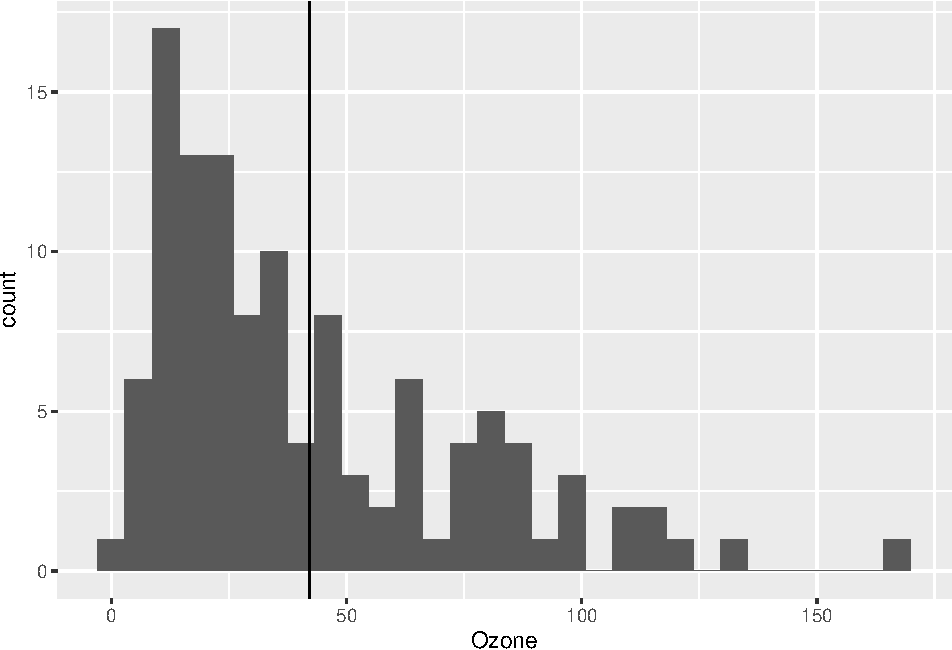
\includegraphics[width=0.5\linewidth]{skeleton_files/figure-latex/unnamed-chunk-2-1} \end{center}

Creating this plot requires greater focus on ggplot2 \emph{syntax},
likely detracting from discussion of \emph{the mean} that statistical
instructors desire.

A syntax that works is as follows:

\begin{Shaded}
\begin{Highlighting}[]
\FunctionTok{library}\NormalTok{(tidyverse)}
\FunctionTok{library}\NormalTok{(magrittr)}

\FunctionTok{ggplot}\NormalTok{(airquality) }\SpecialCharTok{+} 
  \FunctionTok{aes}\NormalTok{(}\AttributeTok{x =}\NormalTok{ Ozone) }\SpecialCharTok{+} 
  \FunctionTok{geom\_histogram}\NormalTok{() }\SpecialCharTok{+} 
  \FunctionTok{geom\_vline}\NormalTok{(}\AttributeTok{xintercept =} 
               \FunctionTok{mean}\NormalTok{(airquality}\SpecialCharTok{$}\NormalTok{Ozone, }
                    \AttributeTok{na.rm =}\NormalTok{ T))}
\end{Highlighting}
\end{Shaded}

\begin{center}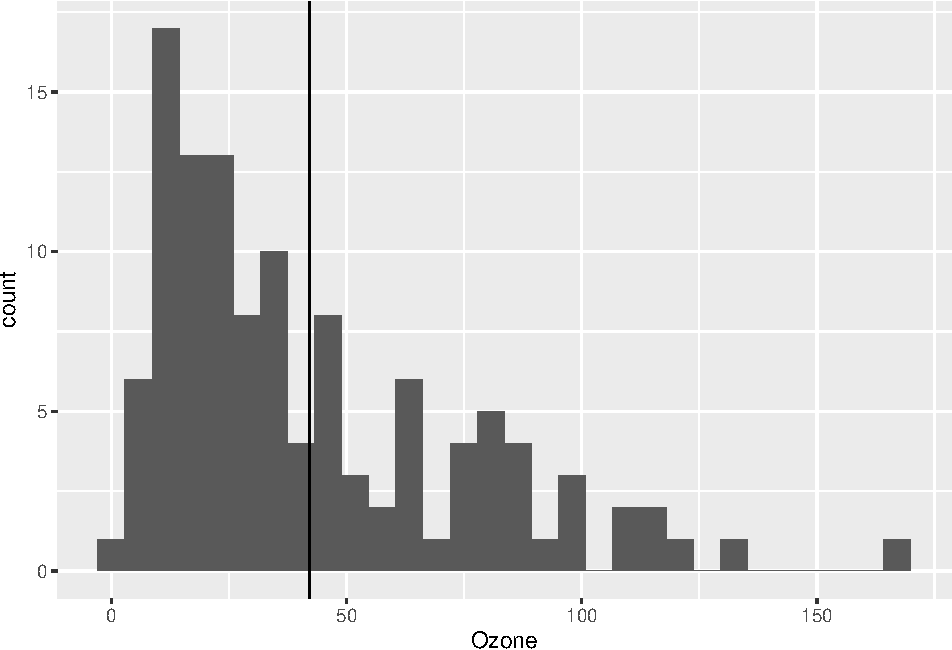
\includegraphics[width=0.5\linewidth]{skeleton_files/figure-latex/unnamed-chunk-3-1} \end{center}

It may require a discussion about dollar sign syntax and how geom\_vline
is actually a special geom -- an annotation -- rather than being mapped
to the data. None of this is relevant to the point you as an instructor
are now forgetting to make: the mean is the balancing point of the data,
or maybe a comment about skewness.

Consider too, the case of wanting to add a vertical line at the mean for
different subsets of the data. This enterprise may take
instructor/analyst/student on an even larger detour -- possibly
googling, and maybe landing on the following stack overflow page where
11,000 souls (some repeats to be sure) have landed:

\url{https://stackoverflow.com/questions/1644661/add-a-vertical-line-with-different-intercept-for-each-panel-in-ggplot2}

The solutions to this problem involve some data manipulation
\emph{prior} to plotting the data. The solution disrupts the forward
flow ggplot build. One must take a pause, which may involve toggling
back and forth between stack overflow solutions, disrupting momentum you
are working on to talk about the pooled mean and the conditional mean.

``Learning becomes less efficient as the mental load students must carry
increases.'' \citep{lovett2000statscongnitive}

Wanda vision ``oh no''
\url{https://media.giphy.com/media/ycBW5N5XMfpXTvamtF/giphy.gif}

\begin{Shaded}
\begin{Highlighting}[]
\NormalTok{airquality }\SpecialCharTok{\%\textgreater{}\%} 
  \FunctionTok{group\_by}\NormalTok{(Month) }\SpecialCharTok{\%\textgreater{}\%} 
  \FunctionTok{summarise}\NormalTok{(}\AttributeTok{Ozone\_mean =} \FunctionTok{mean}\NormalTok{(Ozone, }\AttributeTok{na.rm =}\NormalTok{ T)) }\OtherTok{{-}\textgreater{}}
\NormalTok{airquality\_by\_month}

\FunctionTok{ggplot}\NormalTok{(airquality) }\SpecialCharTok{+} 
  \FunctionTok{aes}\NormalTok{(}\AttributeTok{x =}\NormalTok{ Ozone) }\SpecialCharTok{+} 
  \FunctionTok{geom\_histogram}\NormalTok{() }\SpecialCharTok{+} 
  \FunctionTok{facet\_grid}\NormalTok{(}\AttributeTok{rows =} \FunctionTok{vars}\NormalTok{(Month)) }\SpecialCharTok{+}
  \FunctionTok{geom\_vline}\NormalTok{(}\AttributeTok{data =}\NormalTok{ airquality\_by\_month, }
             \FunctionTok{aes}\NormalTok{(}\AttributeTok{xintercept =} 
\NormalTok{               Ozone\_mean))}
\end{Highlighting}
\end{Shaded}

\begin{center}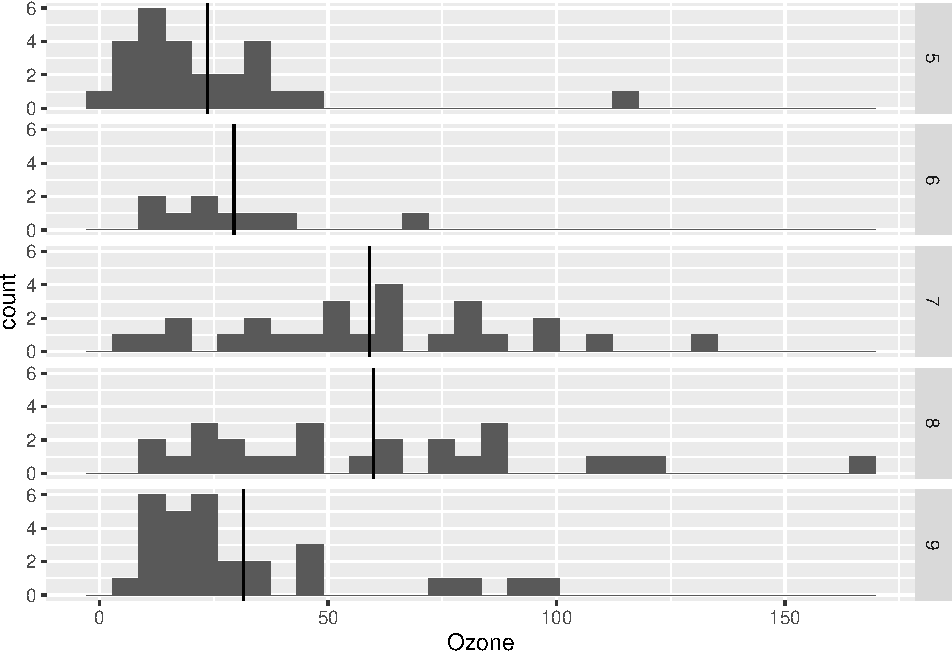
\includegraphics[width=0.5\linewidth]{skeleton_files/figure-latex/unnamed-chunk-4-1} \end{center}

\hypertarget{the-promise}{%
\subsection{The promise}\label{the-promise}}

But, using statistical geometries \emph{can} feel simple. geom\_smooth()
adds loess fit to visualizations in an effortless way; and an ordinary
least squares fit almost as easily. geom\_boxplot reveals a 5-statistic
summary of data medians, the inner quartile range and min/max values in
a single call. The popularity of these easy-to-use functions is evident.
geom\_smooth is used more than 82,000 times in .R and .Rmd files on
GitHub and geom\_boxplot 93,000 times in .R and .Rmd files.

\hypertarget{the-infrastructure-for-extension}{%
\subsection{The infrastructure for
extension}\label{the-infrastructure-for-extension}}

Yet ggplot2 developers and maintainers, with the aim of keeping the code
base robust and reliable, have intentionally limited the out-of-the-box
geoms (as well as other variants) delivered in base ggplot2.

``ggplot2 is already pretty big \ldots{} and it's simply not feasible
for us to include all visualization possibilities into ggplot2 itself.''
- Thomas Pederson
\url{https://www.rstudio.com/resources/rstudioconf-2020/extending-your-ability-to-extend-ggplot2/}

But the extension system is designed to allow for more possibilities.
``It's much better to \ldots{} spread it out on multiple maintainers,
multiple specific packages and so on.''

\url{https://media.giphy.com/media/relSRdIMtKVcPrSfyT/giphy.gif}

Extending ggplot statistical geometries will allow us as teachers,
analysts and students the ease of visual representation for a large
number of other desirable statistical summaries as is experienced with
geom\_boxplot and geom\_smooth.

\hypertarget{introducing-geom_x_mean}{%
\subsection{introducing geom\_x\_mean}\label{introducing-geom_x_mean}}

More geoms for statistical instruction/discussion

\begin{Shaded}
\begin{Highlighting}[]
\FunctionTok{library}\NormalTok{(ggplot2)}
\FunctionTok{ggplot}\NormalTok{(airquality) }\SpecialCharTok{+} 
  \FunctionTok{aes}\NormalTok{(}\AttributeTok{x =}\NormalTok{ Ozone) }\SpecialCharTok{+} 
  \FunctionTok{geom\_histogram}\NormalTok{() }\SpecialCharTok{+} 
\NormalTok{  ggxmean}\SpecialCharTok{::}\FunctionTok{geom\_x\_mean}\NormalTok{() }\SpecialCharTok{+} 
\NormalTok{  ggxmean}\SpecialCharTok{::}\FunctionTok{geom\_x\_median}\NormalTok{(}
    \AttributeTok{linetype =} \StringTok{"dashed"}
\NormalTok{  ) }\SpecialCharTok{+}
  \FunctionTok{scale\_x\_log10}\NormalTok{() }\SpecialCharTok{+}
  \FunctionTok{facet\_grid}\NormalTok{(}\AttributeTok{rows =} \FunctionTok{vars}\NormalTok{(Month)) }\SpecialCharTok{+}
  \FunctionTok{aes}\NormalTok{(}\AttributeTok{color =}\NormalTok{ Month, }\AttributeTok{fill =}\NormalTok{ Month)}
\end{Highlighting}
\end{Shaded}

\begin{center}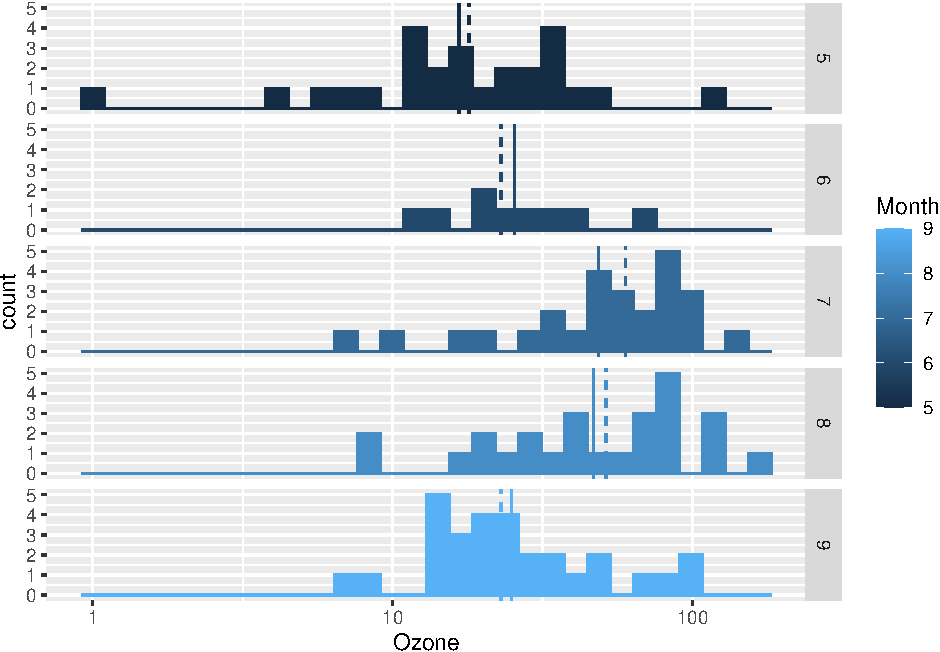
\includegraphics[width=0.5\linewidth]{skeleton_files/figure-latex/unnamed-chunk-5-1} \end{center}

\hypertarget{other-statistical-geometries-in-ggxmean}{%
\subsection{Other statistical geometries in
\{ggxmean\}}\label{other-statistical-geometries-in-ggxmean}}

Beyond providing an easy way to add vertical line at the mean -- and
conditional means, \{ggxmean\} provides a number of other handy geoms!

\hypertarget{annotation-stamps}{%
\subsection{Annotation: Stamps}\label{annotation-stamps}}

\begin{Shaded}
\begin{Highlighting}[]
\FunctionTok{library}\NormalTok{(patchwork)}
\NormalTok{(}\FunctionTok{ggplot}\NormalTok{(}\AttributeTok{data =}\NormalTok{ cars) }\SpecialCharTok{+}
  \FunctionTok{aes}\NormalTok{(dist) }\SpecialCharTok{+}
\NormalTok{  ggxmean}\SpecialCharTok{::}\FunctionTok{stamp\_normal\_dist}\NormalTok{() ) }\SpecialCharTok{/}
\NormalTok{(}\FunctionTok{ggplot}\NormalTok{(}\AttributeTok{data =}\NormalTok{ cars) }\SpecialCharTok{+}
  \FunctionTok{aes}\NormalTok{(dist) }\SpecialCharTok{+}
\NormalTok{  ggxmean}\SpecialCharTok{::}\FunctionTok{stamp\_normal\_prob}\NormalTok{())}
\end{Highlighting}
\end{Shaded}

\begin{center}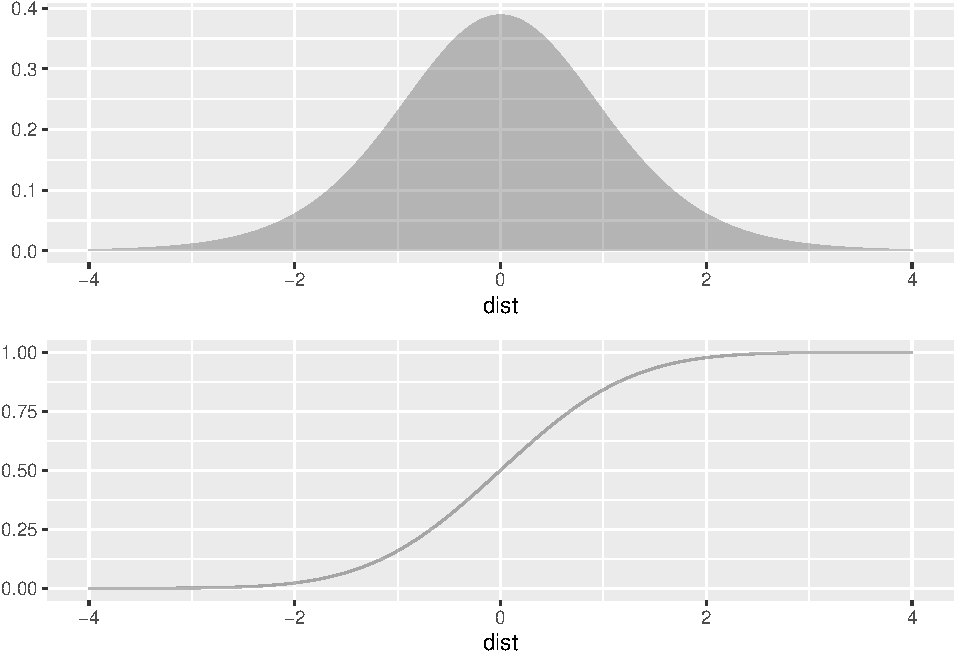
\includegraphics[width=0.5\linewidth]{skeleton_files/figure-latex/unnamed-chunk-7-1} \end{center}

\begin{Shaded}
\begin{Highlighting}[]
\FunctionTok{ggplot}\NormalTok{(}\AttributeTok{data =}\NormalTok{ cars) }\SpecialCharTok{+} 
  \FunctionTok{aes}\NormalTok{(dist) }\SpecialCharTok{+}
\NormalTok{  ggxmean}\SpecialCharTok{::}\FunctionTok{stamp\_normal\_dist}\NormalTok{(}\AttributeTok{fill =} \StringTok{"steelblue"}\NormalTok{) }\SpecialCharTok{+}
\NormalTok{  ggxmean}\SpecialCharTok{::}\FunctionTok{stamp\_t\_dist}\NormalTok{(}\AttributeTok{df =} \DecValTok{4}\NormalTok{,}
               \AttributeTok{fill =} \StringTok{"goldenrod"}\NormalTok{)}
\end{Highlighting}
\end{Shaded}

\begin{center}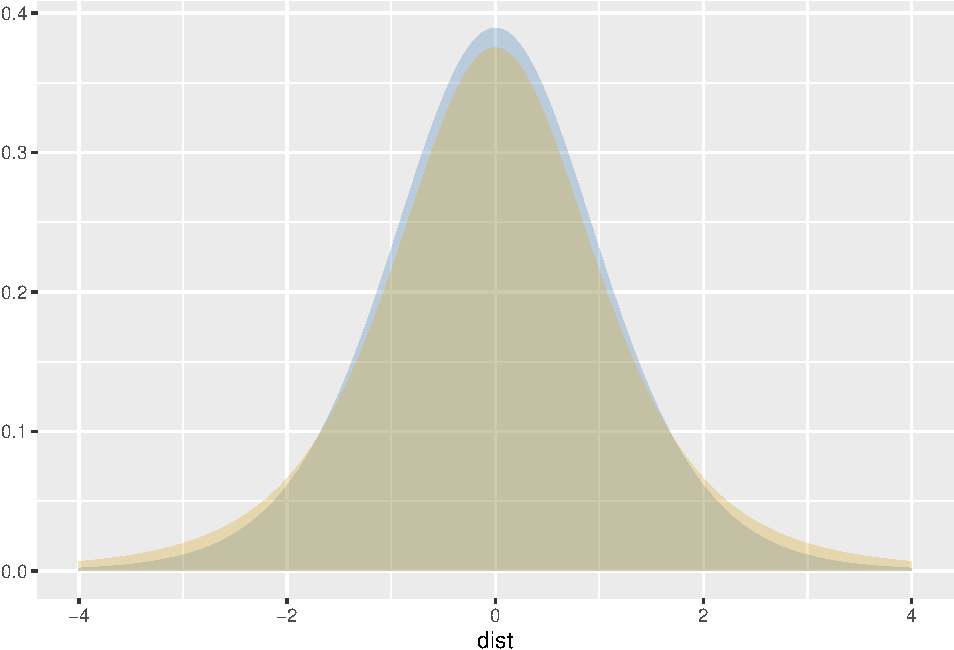
\includegraphics[width=0.5\linewidth]{skeleton_files/figure-latex/unnamed-chunk-8-1} \end{center}

\begin{Shaded}
\begin{Highlighting}[]
\FunctionTok{library}\NormalTok{(patchwork)}
\FunctionTok{library}\NormalTok{(ggplot2)}
\FunctionTok{ggplot}\NormalTok{(cars, }\FunctionTok{aes}\NormalTok{(}\AttributeTok{x =}\NormalTok{ dist)) }\SpecialCharTok{+}
\NormalTok{  ggxmean}\SpecialCharTok{::}\FunctionTok{stamp\_normal\_dist}\NormalTok{(}\AttributeTok{x\_min =} \SpecialCharTok{{-}}\DecValTok{1}\NormalTok{, }\AttributeTok{x\_max =} \DecValTok{1}\NormalTok{, }\AttributeTok{color =} \StringTok{"black"}\NormalTok{, }\AttributeTok{outline.type =} \StringTok{"full"}\NormalTok{) }\SpecialCharTok{+}
\NormalTok{  ggxmean}\SpecialCharTok{::}\FunctionTok{stamp\_normal\_dist}\NormalTok{(}\AttributeTok{x\_min =} \SpecialCharTok{{-}}\DecValTok{2}\NormalTok{, }\AttributeTok{x\_max =} \DecValTok{2}\NormalTok{, }\AttributeTok{color =} \StringTok{"black"}\NormalTok{, }\AttributeTok{outline.type =} \StringTok{"full"}\NormalTok{) }\SpecialCharTok{+}
\NormalTok{  ggxmean}\SpecialCharTok{::}\FunctionTok{stamp\_normal\_dist}\NormalTok{(}\AttributeTok{x\_min =} \SpecialCharTok{{-}}\DecValTok{3}\NormalTok{, }\AttributeTok{x\_max =} \DecValTok{3}\NormalTok{, }\AttributeTok{color =} \StringTok{"black"}\NormalTok{, }\AttributeTok{outline.type =} \StringTok{"full"}\NormalTok{) }\SpecialCharTok{+}
\NormalTok{  ggxmean}\SpecialCharTok{::}\FunctionTok{stamp\_normal\_dist}\NormalTok{(}\AttributeTok{x\_min =} \SpecialCharTok{{-}}\DecValTok{4}\NormalTok{, }\AttributeTok{x\_max =} \DecValTok{4}\NormalTok{, }\AttributeTok{color =} \StringTok{"black"}\NormalTok{, }\AttributeTok{outline.type =} \StringTok{"full"}\NormalTok{) }\SpecialCharTok{+}
\NormalTok{  ggxmean}\SpecialCharTok{::}\FunctionTok{stamp\_normal\_dist}\NormalTok{(}\AttributeTok{x\_min =} \SpecialCharTok{{-}}\DecValTok{5}\NormalTok{, }\AttributeTok{x\_max =} \DecValTok{5}\NormalTok{, }\AttributeTok{color =} \StringTok{"black"}\NormalTok{, }\AttributeTok{outline.type =} \StringTok{"full"}\NormalTok{) }\SpecialCharTok{+}
  \FunctionTok{theme\_classic}\NormalTok{()}
\end{Highlighting}
\end{Shaded}

\begin{center}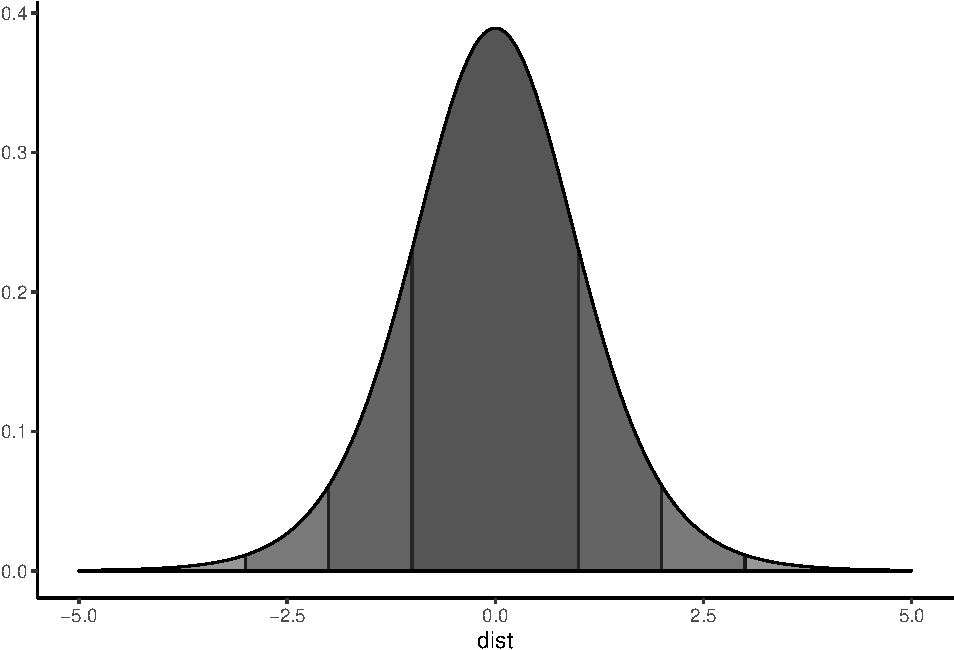
\includegraphics[width=0.5\linewidth]{skeleton_files/figure-latex/unnamed-chunk-9-1} \end{center}

\begin{Shaded}
\begin{Highlighting}[]
\FunctionTok{library}\NormalTok{(patchwork)}
\FunctionTok{ggplot}\NormalTok{(}\AttributeTok{data =}\NormalTok{ cars) }\SpecialCharTok{+}
  \FunctionTok{aes}\NormalTok{(dist) }\SpecialCharTok{+}
\NormalTok{  ggxmean}\SpecialCharTok{::}\FunctionTok{stamp\_chisq\_dist}\NormalTok{(}\AttributeTok{df =} \DecValTok{3}\NormalTok{,}
                   \AttributeTok{fill =} \StringTok{"steelblue"}\NormalTok{) }\SpecialCharTok{+}
\NormalTok{  ggxmean}\SpecialCharTok{::}\FunctionTok{stamp\_chisq\_dist}\NormalTok{(}\AttributeTok{df =} \DecValTok{5}\NormalTok{,}
                   \AttributeTok{fill =} \StringTok{"goldenrod"}\NormalTok{) }\SpecialCharTok{+}
\NormalTok{  ggxmean}\SpecialCharTok{::}\FunctionTok{stamp\_chisq\_dist}\NormalTok{(}\AttributeTok{df =} \DecValTok{7}\NormalTok{,}
                   \AttributeTok{fill =} \StringTok{"plum"}\NormalTok{) }\SpecialCharTok{+}
\NormalTok{  ggxmean}\SpecialCharTok{::}\FunctionTok{stamp\_chisq\_dist}\NormalTok{(}\AttributeTok{df =} \DecValTok{11}\NormalTok{,}
                   \AttributeTok{fill =} \StringTok{"sienna"}\NormalTok{)}
\end{Highlighting}
\end{Shaded}

\begin{center}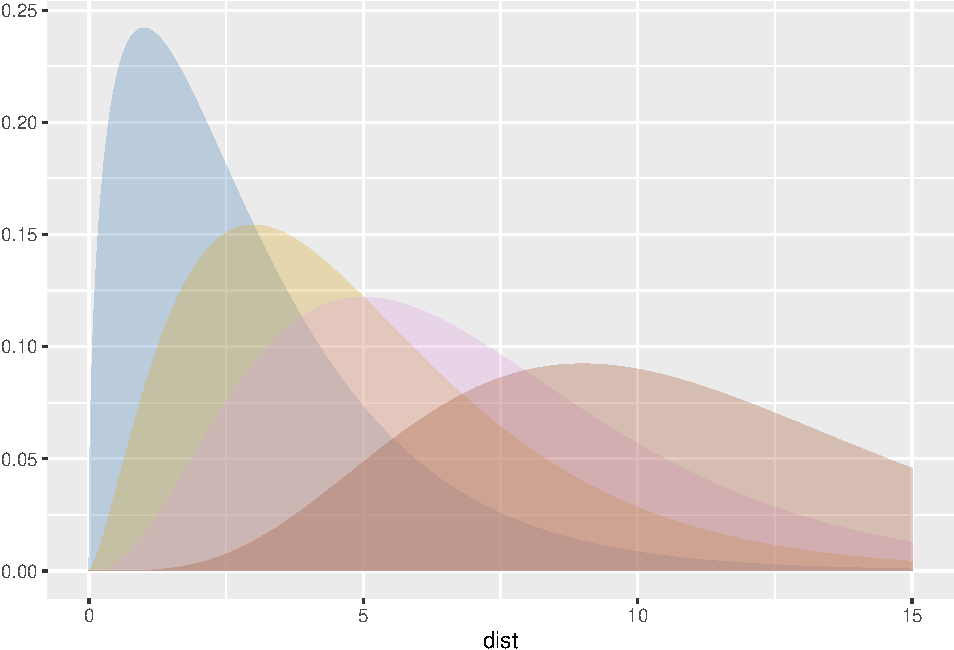
\includegraphics[width=0.5\linewidth]{skeleton_files/figure-latex/unnamed-chunk-10-1} \end{center}

\begin{Shaded}
\begin{Highlighting}[]
\FunctionTok{ggplot}\NormalTok{(}\AttributeTok{data =}\NormalTok{ cars) }\SpecialCharTok{+}
  \FunctionTok{aes}\NormalTok{(dist) }\SpecialCharTok{+}
\NormalTok{  ggxmean}\SpecialCharTok{::}\FunctionTok{stamp\_chisq\_prob}\NormalTok{(}\AttributeTok{df =} \DecValTok{3}\NormalTok{,}
                   \AttributeTok{color =} \StringTok{"steelblue"}\NormalTok{) }\SpecialCharTok{+}
\NormalTok{  ggxmean}\SpecialCharTok{::}\FunctionTok{stamp\_chisq\_prob}\NormalTok{(}\AttributeTok{df =} \DecValTok{5}\NormalTok{,}
                   \AttributeTok{color =} \StringTok{"goldenrod"}\NormalTok{) }\SpecialCharTok{+}
\NormalTok{  ggxmean}\SpecialCharTok{::}\FunctionTok{stamp\_chisq\_prob}\NormalTok{(}\AttributeTok{df =} \DecValTok{7}\NormalTok{,}
                   \AttributeTok{color =} \StringTok{"plum"}\NormalTok{) }\SpecialCharTok{+}
\NormalTok{  ggxmean}\SpecialCharTok{::}\FunctionTok{stamp\_chisq\_prob}\NormalTok{(}\AttributeTok{df =} \DecValTok{11}\NormalTok{,}
                   \AttributeTok{color =} \StringTok{"sienna"}\NormalTok{) }
\end{Highlighting}
\end{Shaded}

\begin{center}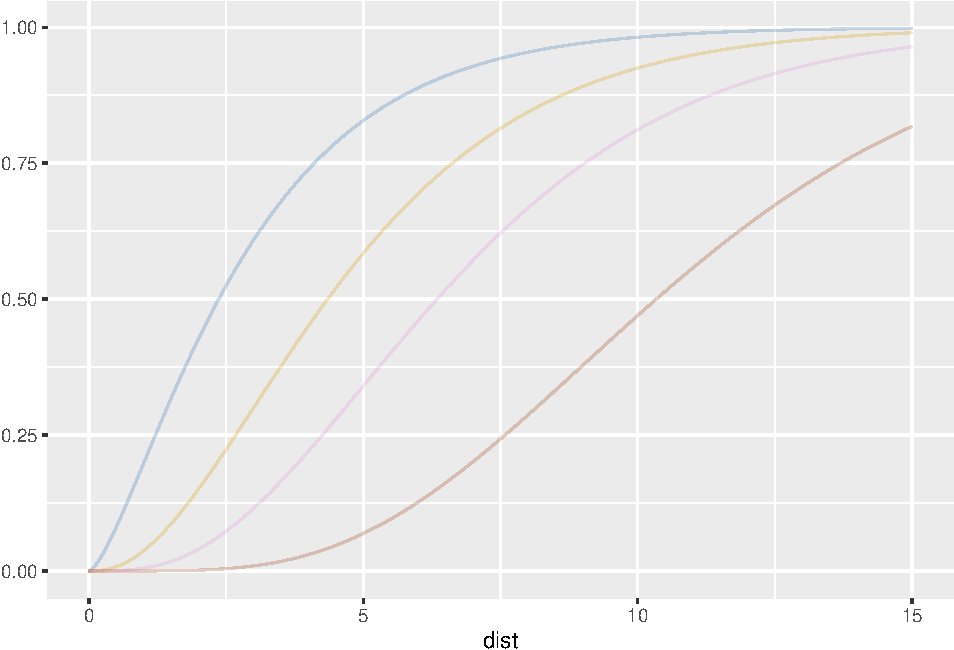
\includegraphics[width=0.5\linewidth]{skeleton_files/figure-latex/unnamed-chunk-10-2} \end{center}

\section{Verifications}
\label{sec:verify}

This section will be just long enough to illustrate what a full page of
text looks like, for margins and spacing.

\citep{tishkovskaya2012statistical}

\bibliographystyle{agsm}
\bibliography{bibliography.bib}

\end{document}
